\section{Part I: The Loom --- The Geometry of Entanglement}

In the prologue, we established a new picture of space: space is not a container, but a fabric woven by wave functions. Now, we must delve into the interior of this loom to see how it works.

\begin{figure}[htbp]
\centering
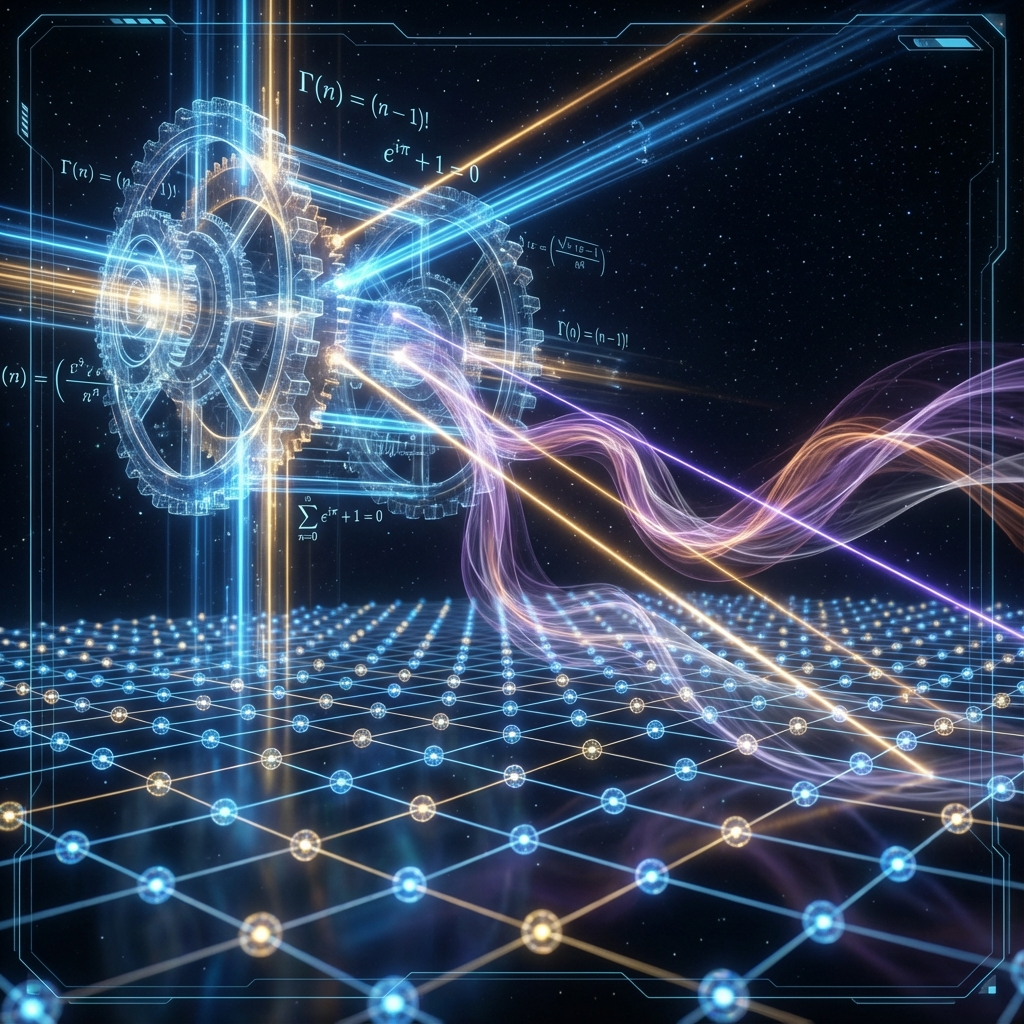
\includegraphics[width=0.8\textwidth]{assets/volume01-introduction/01-00-01-tensor-loom.png}
\caption{Tensor Loom}
\label{fig:tensor-loom}
\end{figure}

If space is a piece of fabric, then this loom is the \textbf{Tensor Network}.

This volume will reveal how the universe uses \textbf{Entanglement Entropy} as glue, bonding discrete qubits (pixels) into continuous geometric space. We will see that the famous \textbf{Area Law} and \textbf{Holographic Principle} are essentially counts of the ``number of thread ends'' in this cosmic fabric.

